% !TEX encoding = UTF-8 Unicode
% -*- coding: UTF-8; -*-
\ifdefined\ishandout
\documentclass[handout]{beamer}
\else
\documentclass[11pt]{beamer}
\fi

\usepackage[frenchb]{babel}
\usepackage[T1]{fontenc}
\usepackage[utf8]{inputenc}
\usepackage{hyperref}
\usepackage{multirow}
\usepackage{listings}
\usepackage{fancyvrb}
\usepackage{tikz}
\usepackage{framed}
\usepackage{algorithm}
\usepackage{algorithmic}
\usepackage{xcolor}
\usepackage{color, colortbl}
\ifdefined\ishandout
\usepackage{handoutWithNotes}
\fi
\usepackage{slashbox}
\usepackage{amsmath}
\usepackage{bm}
\usepackage{hhline}
\usepackage{xmpmulti}

\usetikzlibrary{shapes.geometric}
\usetikzlibrary{positioning}
\usetikzlibrary{shapes.arrows, chains}
\usetikzlibrary{arrows,calc}
\usetikzlibrary{shapes.multipart}
\usepackage{array}
\usetheme{Boadilla}

\usefonttheme[onlymath]{serif}

\newcommand{\R}{\mathbb{R}}
\newcommand{\C}{\mathbb{C}}
\newcommand{\N}{\mathbb{N}}
\newcommand{\Z}{\mathbb{Z}}
\newcommand{\E}{\mathbb{E}}
\newcommand{\Var}{\text{Var}}
\newcommand{\Cov}{\text{Cov}}
\ifdefined\ishandout
\pgfpagesuselayout{3 on 1 with notes}[a4paper,border shrink=5mm]
\usecolortheme{dove}
\else
%\usecolortheme{dolphin}
\usecolortheme{beaver}
\fi


\lstnewenvironment{codeC}
{ \lstset{language=C,
    otherkeywords={printf,scanf}}
}
{}

\ifdefined\ishandout
\definecolor{mygreen}{rgb}{0,0,0}
\definecolor{mymauve}{rgb}{0,0,0}
\definecolor{myblue}{rgb}{0,0,0}
\else
\definecolor{mygreen}{rgb}{0,0.6,0}
\definecolor{mymauve}{rgb}{0.58,0,0.82}
\definecolor{myblue}{rgb}{0,0,1}

\fi

%% Notes
%\setbeameroption{show only notes}


\definecolor{mygray}{rgb}{0.5,0.5,0.5}

\lstset{ language=Python,%
  backgroundcolor=\color{white},   % choose the background color; you must add \usepackage{color} or \usepackage{xcolor}
  basicstyle=\footnotesize,        % the size of the fonts that are used for the code
  breakatwhitespace=false,         % sets if automatic breaks should only happen at whitespace
  breaklines=true,                 % sets automatic line breaking
  captionpos=b,                    % sets the caption-position to bottom
  commentstyle=\color{mygreen},    % comment style
  deletekeywords={...},            % if you want to delete keywords from the given language
  escapeinside={\%*}{*)},          % if you want to add LaTeX within your code
  extendedchars=true,              % lets you use non-ASCII characters; for 8-bits encodings only, does not work with UTF-8
  frame=tb,	                   % adds a frame around the code
  keepspaces=true,                 % keeps spaces in text, useful for keeping indentation of code (possibly needs columns=flexible)
  keywordstyle=\color{blue},       % keyword style
  otherkeywords={*,...},           % if you want to add more keywords to the set
  numbers=none,                    % where to put the line-numbers; possible values are (none, left, right)
  numbersep=5pt,                   % how far the line-numbers are from the code
  numberstyle=\tiny\color{mygray}, % the style that is used for the line-numbers
  rulecolor=\color{black},         % if not set, the frame-color may be changed on line-breaks within not-black text (e.g. comments (green here))
  showspaces=false,                % show spaces everywhere adding particular underscores; it overrides 'showstringspaces'
  showstringspaces=false,          % underline spaces within strings only
  showtabs=false,                  % show tabs within strings adding particular underscores
  stepnumber=2,                    % the step between two line-numbers. If it's 1, each line will be numbered
  stringstyle=\color{mymauve},     % string literal style
  tabsize=3,	                   % sets default tabsize to 2 spaces
  title=\lstname                   % show the filename of files included with \lstinputlisting; also try caption instead of title
}
%\lstset{language=Python,
% breakatwhitespace=false,         % sets if automatic breaks should only happen at whitespace
%  breaklines=true,                 % sets automatic line breaking
%  captionpos=b,                
%%commentstyle=\itshape\color{mymauve},
%%keywordstyle=\bfseries\color{myblue},
%numbers=left,                    % where to put the line-numbers; possible values are (none, left, right)
%  numbersep=8pt,                   % how far the line-numbers are from the code
%  numberstyle=\tiny\color{mygray}, % the style that is used for the line-numbers
%%  rulecolor=\color{black},         % if not set, the frame-color may be changed on line-breaks within not-black text (e.g. comments (green here))
%  showspaces=false,                % show spaces everywhere adding particular underscores; it overrides 'showstringspaces'
%%  showstringspaces=false,          % underline spaces within strings only
%  showtabs=false,                  % show tabs within strings adding particular underscores
%  stepnumber=2,                    % the step between two line-numbers. If it's 1, each line will be numbered
%%  stringstyle=\color{mygreen},     % string literal style
%  tabsize=2 
%}
\ifdefined\ishandout
\newcommand{\red}{\textbf}
\else
\newcommand{\red}{\textcolor{red}}
\fi
%\newcommand \emph
%Default size : 12.8 cm * 9.6 cm

\newcommand{\tmark}[1]{\tikz[remember picture, baseline=-.5ex]{\coordinate(#1);}}

\ifdefined\ishandout
\newenvironment<>{codeblock}[1]{%begin
  \setbeamercolor{block title}{fg=black,bg=lightgray!80}%
  \begin{block}{#1}}
  % \begin{codeC}}
  %  {\end{codeC}
{  
\end{block}}

\newenvironment<>{termblock}[1]{
    \setbeamercolor{block title}{fg=black,bg=lightgray!90}%
    \begin{block}{#1}
}
%     \begin{Verbatim}}
{%\end{Verbatim}
\end{block}
}

\definecolor{bluegreen}{RGB}{0,0,0}
%\definecolor{bluegreen}{rgb}{0,0.6,0.8}
\else

\newenvironment<>{codeblock}[1]{%begin
  \setbeamercolor{block title}{fg=darkgray,bg=yellow}%
  \begin{block}{#1}}
  % \begin{codeC}}
  %  {\end{codeC}
{  
\end{block}}

\newenvironment<>{termblock}[1]{
    \setbeamercolor{block title}{fg=white,bg=lightgray}%
    \begin{block}{#1}}
%     \begin{Verbatim}}
{%\end{Verbatim}
\end{block}
}

\definecolor{bluegreen}{RGB}{0,149,182}
%\definecolor{bluegreen}{rgb}{0,0.6,0.8}
\fi

%\newcommand{\output}[1]{
\setbeamertemplate{navigation symbols}{}
\newcommand{\bvrb}{\Verb[commandchars=£µ§,formatcom=\color{bluegreen}]}
\newcommand{\footvrb}{\footnotesize\Verb}
\newcommand{\vrbalert}[2][]{\visible<#1>{#2}}
%%% Commande pour les listes/arbres
\newcommand{\mvide}{\nodepart{one} \nodepart{two}}
\newcommand{\tvide}{\nodepart{one} \nodepart{two} \nodepart{three}}
\newcommand{\rref}[1][]{\hfill{\scriptsize\textit{#1}}}

%%Fin des commandes pour les listes/arbres.

\setbeamerfont{caption}{size=\scriptsize}

%%% Paramètres du cours (à régler)
%Numéro du cours
\newcommand{\nb}{1}

\title[Machine learning]{Reconstructing and forecasting oceanic key variables using data-driven algorithms}
\author[J. Brajard]{julien.brajard@upmc.fr}
\institute[LOCEAN/UPMC]{LOCEAN-UPMC}
\date{30 May 2017}
\begin{document}
%%%%%%%%%%%%%%%%%%%%% SLIDES DE TITRE
\begin{frame}
\titlepage
%\centering{
%\url{http://australe.upmc.fr} (onglet EPU-C5-IGE Info Gen)}
\end{frame}


%%%%%%%%%%%%%%%%%%%%%%
\begin{frame}
\frametitle{Different types of problems}
What are the \red{methological} problems associated with earth
observations data ?
\begin{itemize}
\item Prediction (data completion, hidden variables)
\item Forecasting 
\item Classification
\end{itemize}
\end{frame}

%%%%%%%%%%%%%%%%%%%%%%
\begin{frame}
\frametitle{Example of prediction}
\framesubtitle{Data completion}
\begin{figure}
\includegraphics[width=0.9\textwidth]{./fig/chlor_a-VIIRS-15May2017.png}
\caption{Chlorophyll-a concentration (15 May 2017) by sensor VIIRS}
\end{figure}
\end{frame}


%%%%%%%%%%%%%%%%%%%%%%
\begin{frame}
\frametitle{Example of forecast}
Forecast of Total Suspended Matter (TSM) in a time future.
\begin{columns}
\column{.45\textwidth}
\begin{figure}
%\transduration<0-10>{0}
% \multiinclude[<+->][format=png,
% graphics={width=\textwidth}]{fig/carte-tsm}
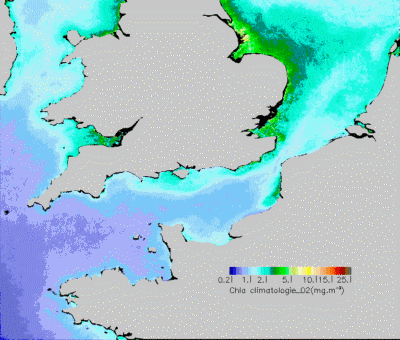
\includegraphics[width=0.9\textwidth]{./fig/carte-tsm-0.png}

\end{figure}
\column{.45\textwidth}
\begin{figure}
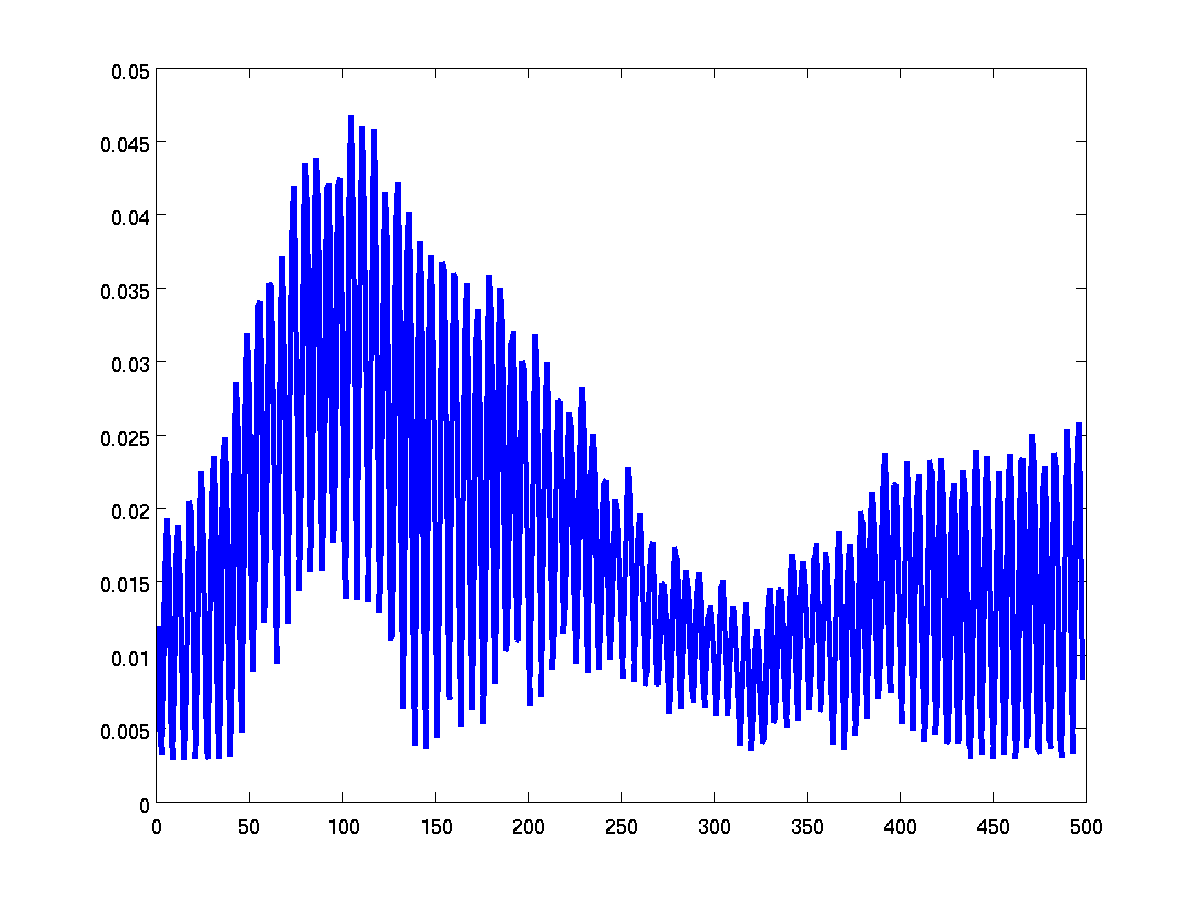
\includegraphics[width=0.9\textwidth]{./fig/serie-temp-tsm.png}
\caption{Temporal evolution of TSM for a pixel}
\end{figure}

\column{.1\textwidth}
$\rightarrow$ ?
\end{columns}
\end{frame}

%%%%%%%%%%%%%%%%%%%%%
\begin{frame}
\frametitle{Example of classification}
\framesubtitle{Bio-region in Mediterranean Sea}
\begin{figure}
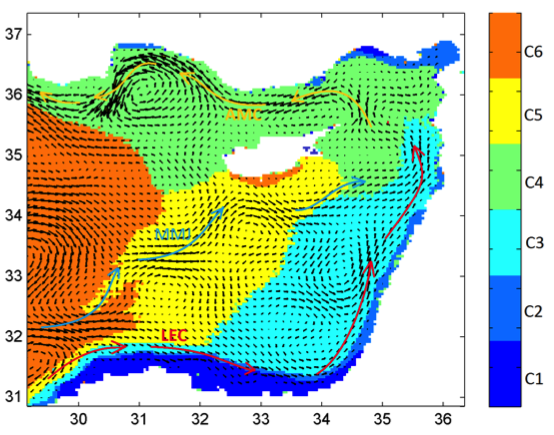
\includegraphics[width=0.6\textwidth]{./fig/bioregions.png}
\caption{Classification of East-Mediterranean using chlorophyll-a
  concentration and surface temperature seasonal cycles}
\end{figure}
\vspace{-1em}
\rref[Hourani et al. (2017)]
\end{frame}

%%%%%%%%%%%%%%%%%%%%%
\begin{frame}
\frametitle{Why using machine learning ?}
\begin{enumerate}
\begin{columns}[t]
\column{.45\textwidth}
\item Number of observation data is continuously increasing
\begin{figure}
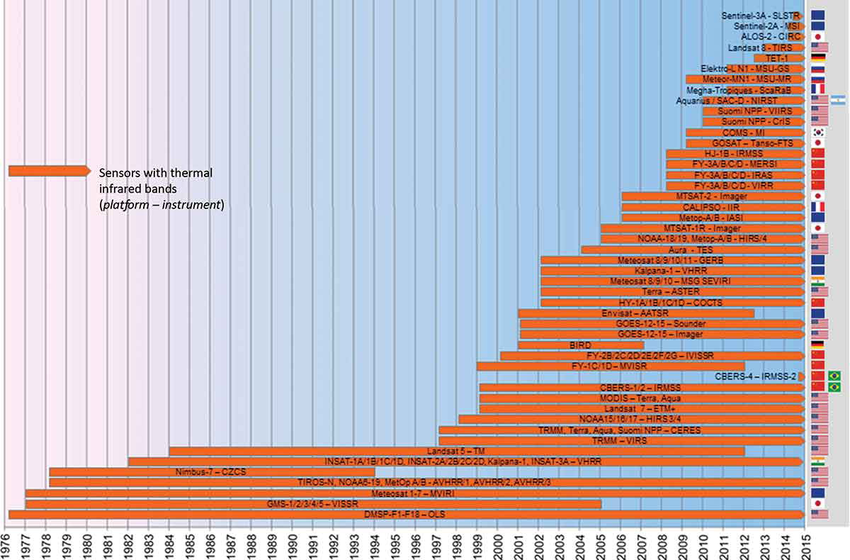
\includegraphics[width=0.9\textwidth]{./fig/sat-sst.png}
\caption{Satellites providing semi-global and daily coverage of surface
temparture}
\end{figure}
\rref[Kuenzer et al. (2014)]
\pause
\column{.45\textwidth}
\item Performances of machine learning algorithm are improving
\begin{figure}
\includegraphics[width=0.9\textwidth]{./fig/object-recognition.pdf}
\caption{image recognition performances}
\end{figure}
\end{columns}
\end{enumerate}
\end{frame}

%%%%%%%%%%%%%%%%%%%%%
\begin{frame}
\frametitle{Definition of machine learning}
\begin{columns}
\column{.5\textwidth}
Machine learning consists in defining
\begin{itemize}
\item Some data to work on and expected outputs.
\item A computational architecture (the \red{machine})
\item A \red{learning} process (estimation of control parameters).
\end{itemize}
\pause
\column{.5\textwidth}
\begin{figure}
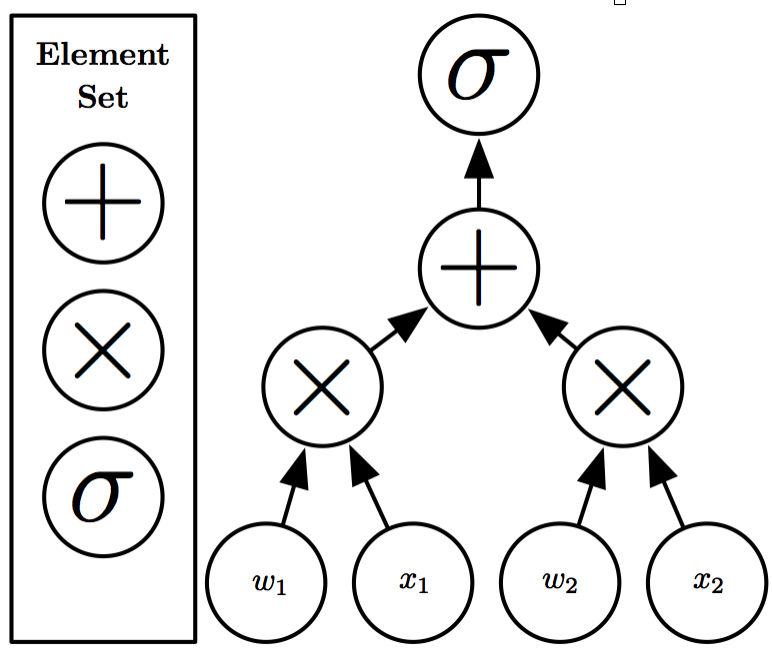
\includegraphics[width=0.9\textwidth]{./fig/computation-graph.png}
\caption{Elementary computation. $x_i$ are the input parameters and
  $w_i$ are control parameters to "learn" (i.e. to optimally estimate).}
\end{figure}
\rref[Goodfellow (2016)]

\end{columns}
\end{frame}

%%%%%%%%%%%%%%%%%%%%%%%%
\begin{frame}
\frametitle{Example(1): the linear regression}
The linear regression is an example of machine learning
$$ y = w_1 . x_1$$
$x_1$ is the input data and $w_1$ is a control parameter.
\begin{figure}
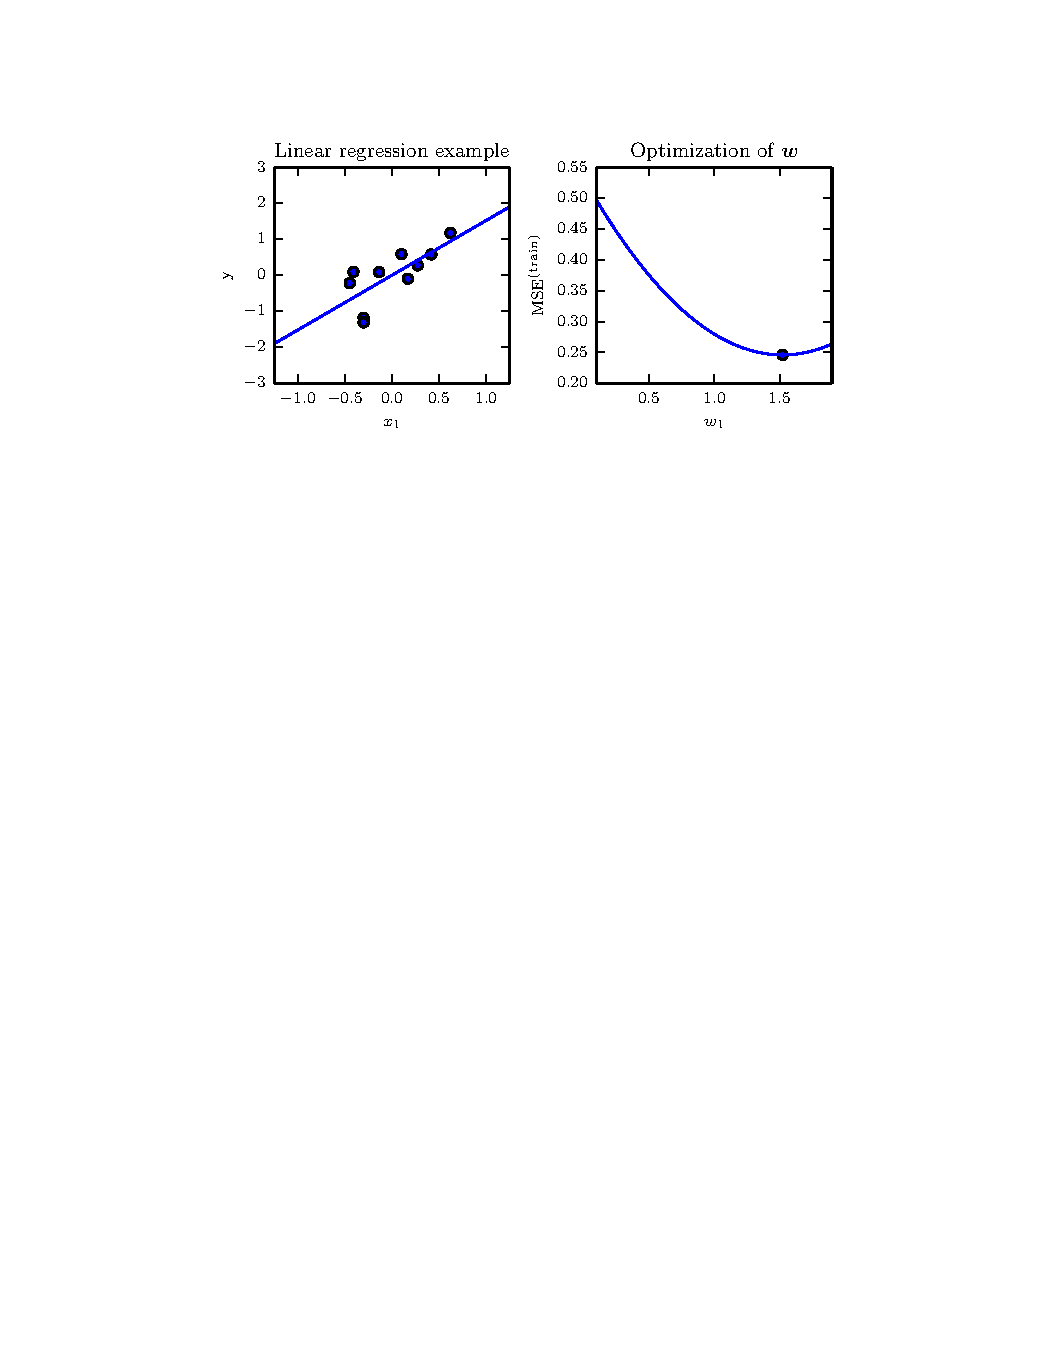
\includegraphics[width=0.9\textwidth]{./fig/linear-reg.pdf}
\end{figure}
\rref[Goodfellow (2016)]

\end{frame}


%%%%%%%%%%%%%%%%%%%%%
\begin{frame}
\frametitle{Example(2):  the multilayer perceptron}
We can concatenate several elementary computational graphs
\begin{figure}
\includegraphics[width=0.5\textwidth]{./fig/mlp.jpg}
\caption{Each arrow of the network is weighted by a control parameter $w$}
\end{figure}
The parameters are trainable using the "gradient backpropagation aglorithm"
\end{frame}

%%%%%%%%%%%%%%%%%%%%%%%%
\begin{frame}
\frametitle{Complexity of a neural networks}
\begin{columns}
\column{.5\textwidth}
\begin{figure}
\includegraphics[width=1\textwidth]{./fig/connections.pdf}
\caption{Evolution of connection by neurons for various neural networks}
\end{figure}
\column{.5\textwidth}
\begin{figure}
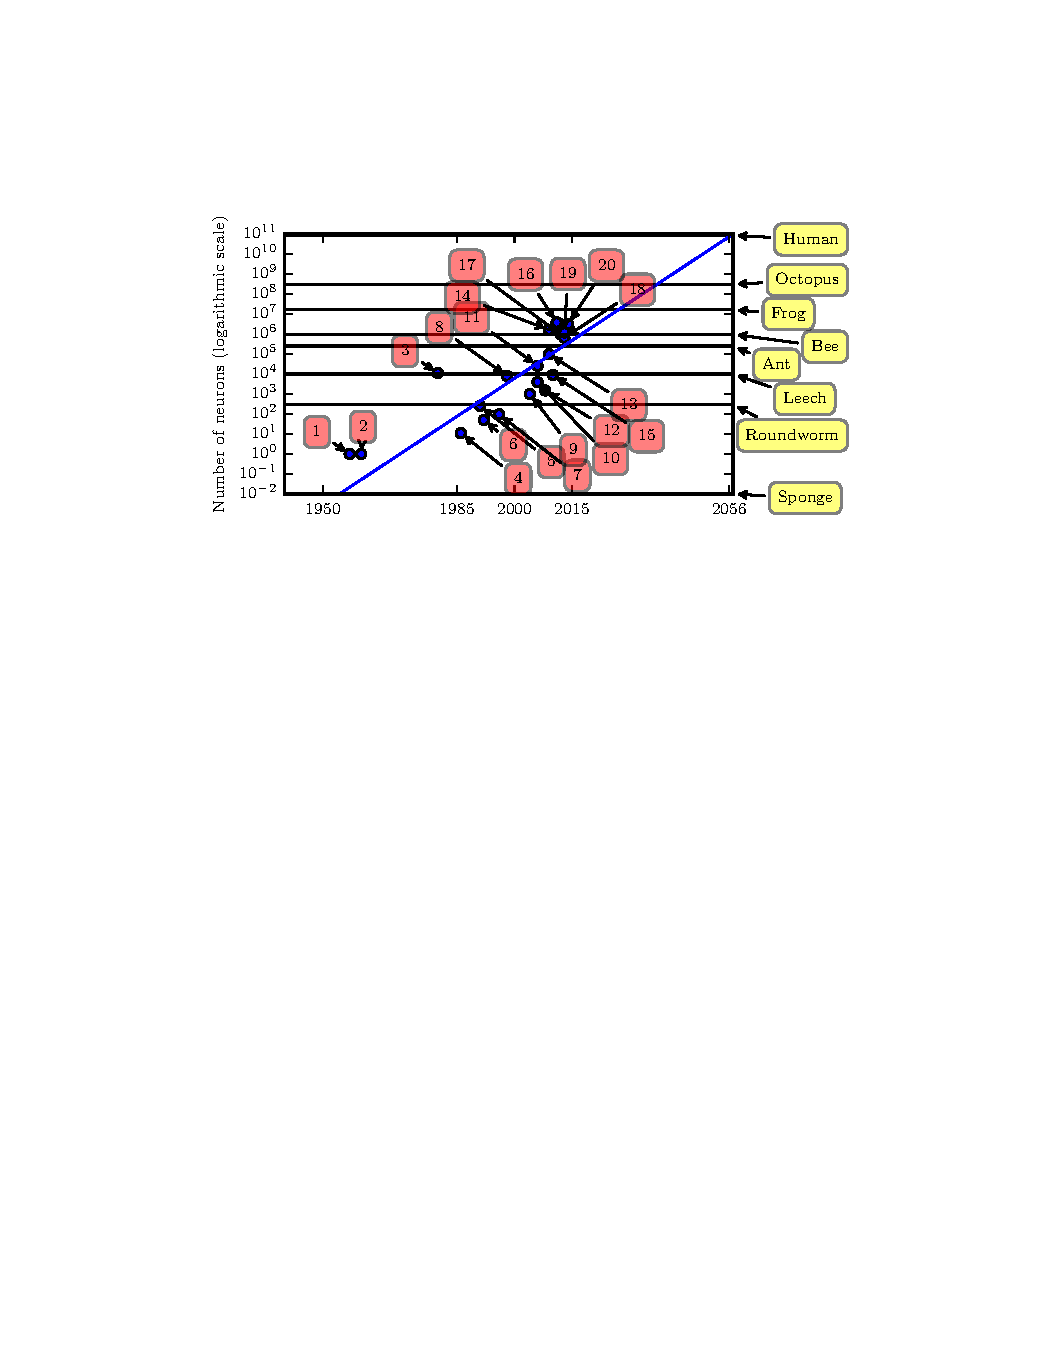
\includegraphics[width=1\textwidth]{./fig/neurons.pdf}
\caption{Evolution of number of neurons for various neural networks}
\end{figure}
\end{columns}
\rref[Goodfellow (2016)]\\
\end{frame}

%%%%%%%%%%%%%%%%%%%%%%%%%
\begin{frame}
\frametitle{An application: reconstructing subsurface velocities}
\begin{figure}
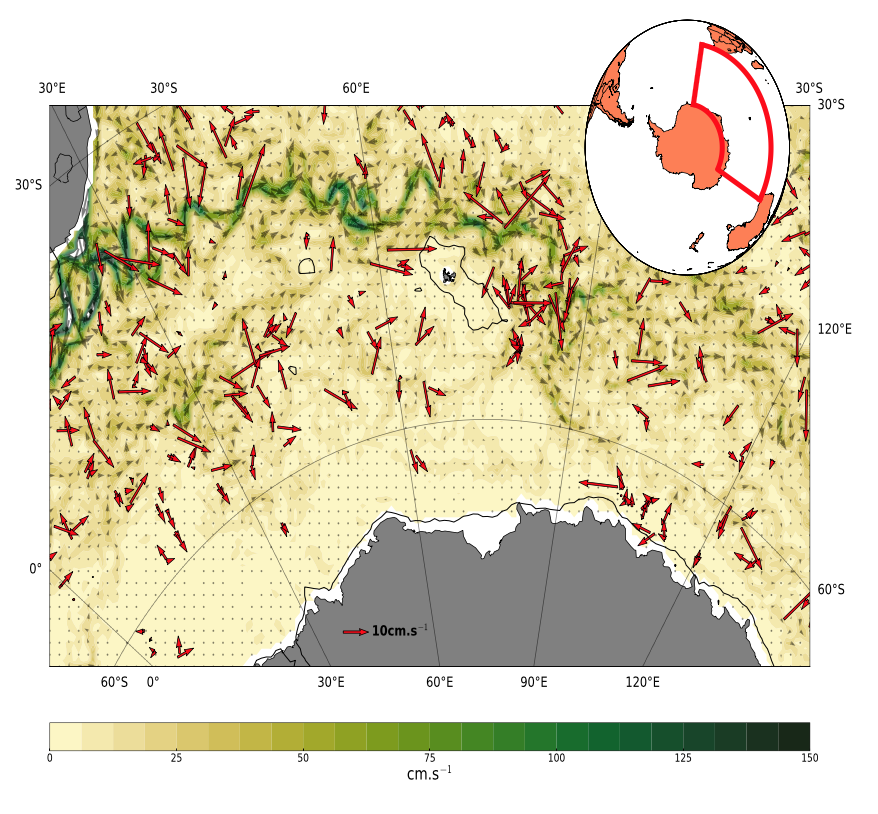
\includegraphics[width=0.5\textwidth]{./fig/illustration-depth.png}
\caption{Surface velocity from altimetry (color and black arrow) and
  velocity at 1000m (red arrow) from ARGO floats on April 17,2009}
\end{figure}
\rref[Chapman and Charantonis (2017)]
\end{frame}

%%%%%%%%%%%%%%%%%%%%%%%%%
\begin{frame}
\frametitle{Architecture of the neural network}
\begin{figure}
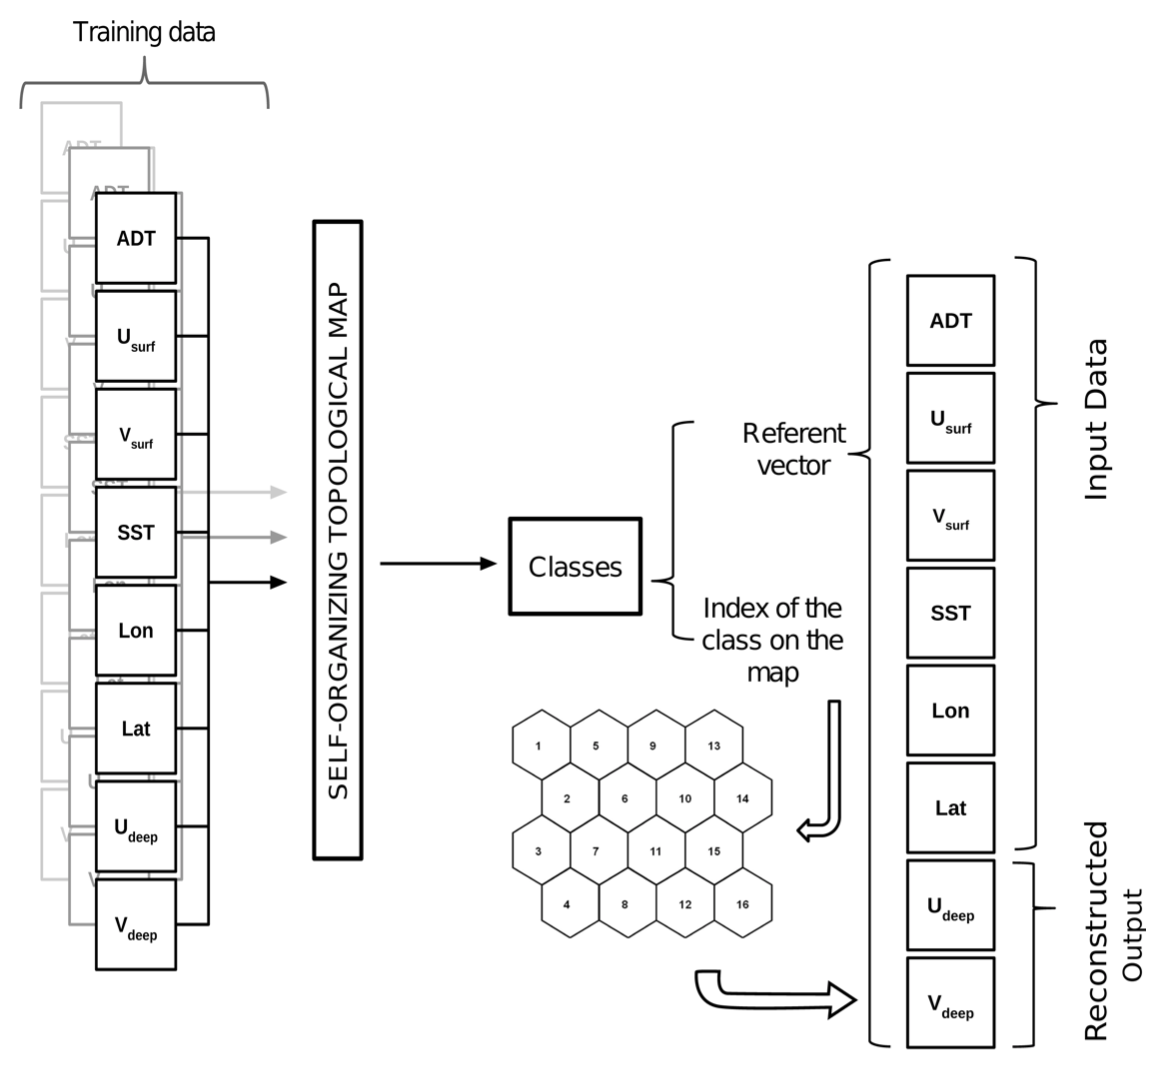
\includegraphics[width=0.6\textwidth]{./fig/schema-method.png}
\end{figure}
\end{frame}


%%%%%%%%%%%%%%%%%%%%%%%%%
\begin{frame}
\frametitle{Results}
\begin{columns}
\column{.5\textwidth}
\begin{figure}
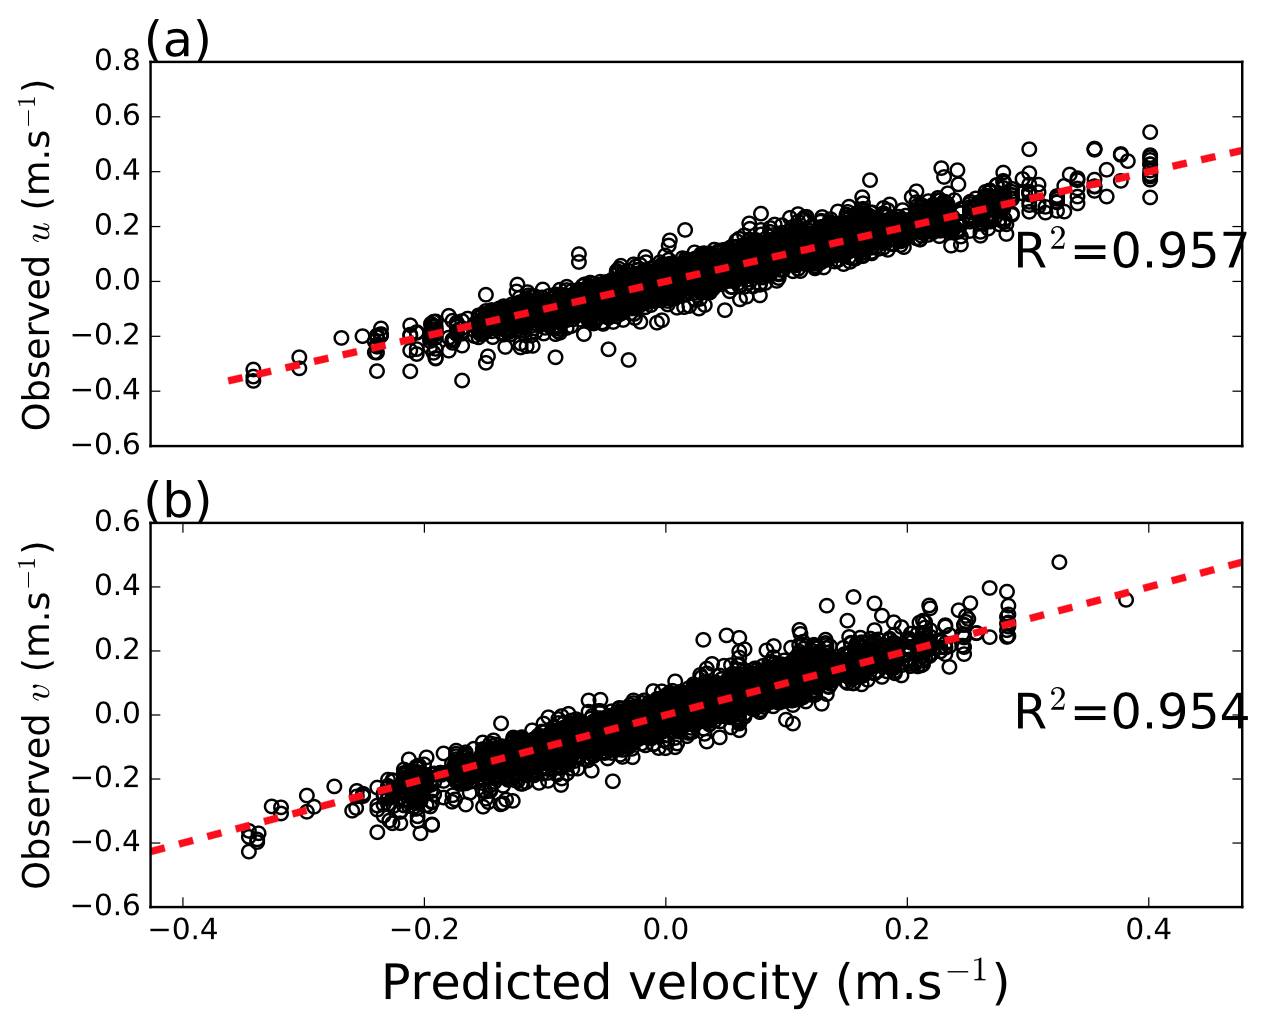
\includegraphics[width=0.9\textwidth]{./fig/scatter-depth.png}
\caption{Observed subsurface velocity with respect to the reconstructed
  subsurface velocity} 
\end{figure}
\pause
\column{.5\textwidth}
\begin{figure}
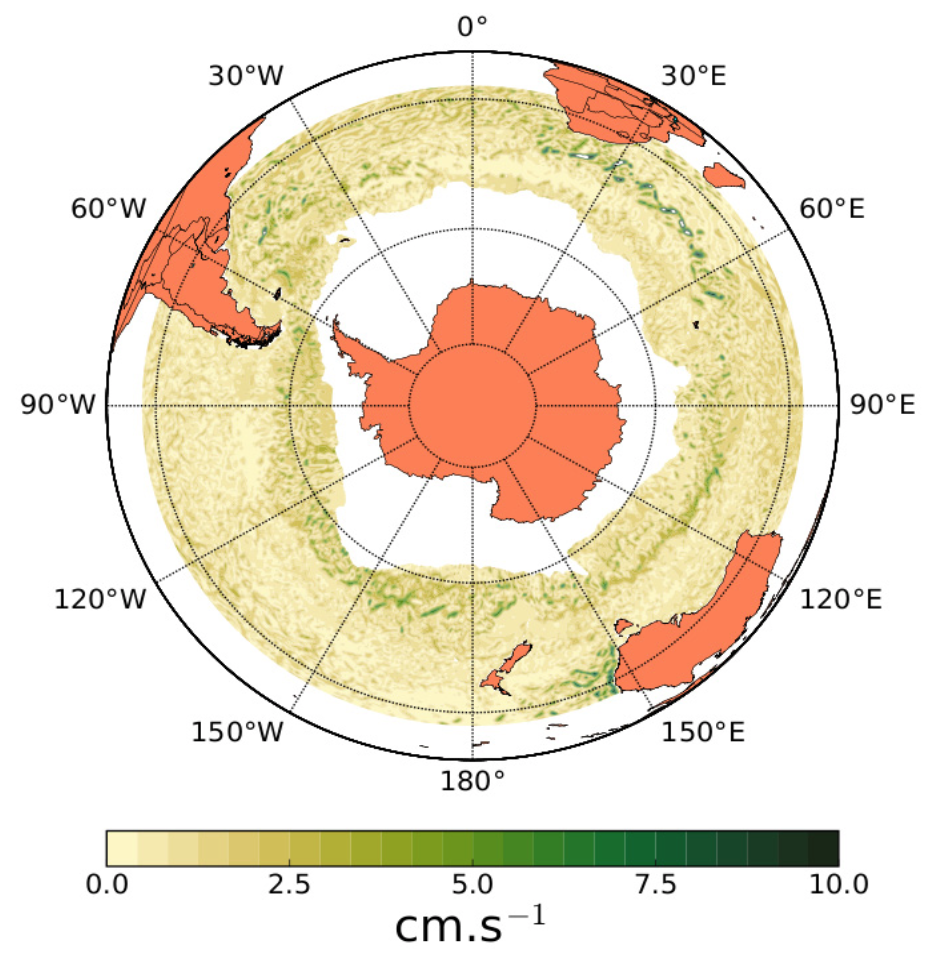
\includegraphics[width=0.9\textwidth]{./fig/depth-vel.png}
\caption{Time mean reconstructed velocity at 1000m depth in 2009.} 
\end{figure}
\end{columns}
\end{frame}


%%%%%%%%%%%%%%%%%%%%%%%%%%
\begin{frame}
\frametitle{Conclusions}
\begin{itemize}[<+->]
\item Machine learning approach is relevant to reconstruct unobserved
  data from earth observation data
\item Despite the maturity of meachine learning, methodologies
  specific to environmental science are still to be found
\item How to use the complementary between the knowledge extracted from data
and the physical and numerical models ?
\end{itemize}
\end{frame}


\end{document}